\documentclass[11pt,a4paper]{article}
\usepackage[margin=0.82in]{geometry}
\usepackage{amsmath,amssymb,bm,booktabs,graphicx,microtype}
\usepackage[colorlinks=true,urlcolor=blue,linkcolor=blue]{hyperref}
\setlength{\parindent}{0pt}
\setlength{\parskip}{5pt}
\newcommand{\N}{\mathsf N}
\begin{document}
\begin{center}
{\Large\bfseries A nonzero interacting Jordan pole\\in a spin-symmetric Anderson control}\\[5pt]
Research calculation for review --- 28 October 2026
\end{center}

\textbf{Finding.} A half-filled Anderson dimer with an imposed local PT field
has a nonzero impurity Green-function double pole for every finite repulsive
$U$ and nonzero hopping. Untruncated calculations with three and five bath
sites also verify selected interacting double poles. This closes the
\emph{residue-amplitude} gap in the existing symmetry-control audit; it does
not solve the original driven, spin-asymmetric continuum problem.

\section*{1. Model, state and conditional residue theorem}
Let $H_A$ be a spin-rotation-invariant Anderson Hamiltonian with scalar bath
hopping and hybridization, impurity energy $\epsilon_d$, and local interaction
$Un_{d\uparrow}n_{d\downarrow}$. Add a field only on the impurity:
\begin{equation}
 H=H_A+d^\dagger\N d,\qquad
 \N=\Delta\sigma_x+i\gamma\sigma_z,\qquad
 \N^2=(\Delta^2-\gamma^2)I .
\end{equation}
Here $d=(d_\uparrow,d_\downarrow)^T$, $\Delta,\gamma$ are real energies, and
$\sigma_+=(\sigma_x+i\sigma_y)/2$. The antiunitary symmetry is internal
spin exchange followed by complex conjugation, not the physical spin
time-reversal operator of an arbitrary SOC host. At $\gamma=\Delta>0$,
$\N\ne0$ is nilpotent; a unitary spin rotation maps it to
$2\Delta\sigma_+$. No Green function or self-energy is fitted to this form.

For a finite bath, assume an isolated spin-singlet reference ground state
of $H_A$. Define the response by analytic continuation of that state, using
left and right eigenvectors with $\langle L|R\rangle=1$; $Q$ denotes its
particle number and $H_q$ the restriction to charge sector $q$:
\begin{align}
G_{ab}(z)={}&\langle L|d_a(z+E_0-H_{Q+1})^{-1}d_b^\dagger|R\rangle\nonumber\\
 &+\langle L|d_b^\dagger(z-E_0+H_{Q-1})^{-1}d_a|R\rangle .
\end{align}
This is a biorthogonal meromorphic response. It is not a claim about a
thermal or pumped steady state of a gain--loss experiment.

\textbf{Proposition.} For an isolated addition spin doublet, let $\omega_\alpha$
be its transition energy at zero field, $Z_\alpha$ its per-spin impurity
spectral weight, and
$m_\alpha=\partial_h\omega_{\alpha,\uparrow}(h)|_{h=0}$ the slope under a
real local field $h(n_{d\uparrow}-n_{d\downarrow})$. At the null field,
\begin{equation}
 G(z)=g_0(z)I+g_1(z)\N,\qquad
 B_\alpha\equiv\mathop{\rm Res}_{z=\omega_\alpha}
 [(z-\omega_\alpha)G(z)]=Z_\alpha m_\alpha\N .
 \label{eq:residue}
\end{equation}
Thus $Z_\alpha m_\alpha\ne0$ proves a double pole, whereas alignment with
$\N$ alone does not. For $K=G^{-1}$ this also gives the nonlinear pole
certificate:
\begin{equation}
 K(\omega_\alpha)=-\frac{m_\alpha}{Z_\alpha}\N,\qquad
 \det K=\frac{(z-\omega_\alpha)^2}{Z_\alpha^2}
        +O((z-\omega_\alpha)^3).
\end{equation}
Thus $K$ has rank one, $F=F'=0$, and $F''=2/Z_\alpha^2\ne0$ for
$F=\det K$ at the pole.

\textbf{Derivation.} Complex-spin covariance constrains the response to
$g_0(z,u)I+g_1(z,u)\N$, with $u=\bm B\cdot\bm B$ and
$\bm B=(\Delta,0,i\gamma)$. At $u=0$, $g_0$ is the
zero-field Green function and $g_1=\partial_hG_{\uparrow\uparrow}(z,h)|_0$.
Differentiating $Z_\alpha(h)/[z-\omega_\alpha(h)]$ gives a double-pole term
$Z_\alpha m_\alpha/(z-\omega_\alpha)^2$ and a simple-pole term from
$\partial_hZ_\alpha$. Analytic continuation along the null field is allowed
while the singlet remains isolated. Covariance alone supplies no general
lower bound on $Z_\alpha m_\alpha$ for arbitrary baths.

\newpage
\section*{2. Analytic finite-$U$ result at single occupancy}
Take one spinful bath site at energy zero, hopping $V>0$, and
$\epsilon_d=-U/2$, with chemical potential zero. Define
\begin{equation}
 A=\sqrt{U^2/16+V^2},\quad C=\sqrt{U^2/16+4V^2},\quad
 \omega_\ell=C-A,\quad\omega_h=C+A .
\end{equation}
The singlet energy is $E_0=-U/4-C$. Direct diagonalization gives
\begin{align}
g_0(z)&=\left[z-\frac{V^2}{z}
                -\frac{U^2}{4}\frac{z}{z^2-9V^2}\right]^{-1},\label{eq:g0}\\
Z_\ell&=\frac{\omega_\ell^2-9V^2}
                   {2(\omega_\ell^2-\omega_h^2)},\qquad
m_\ell=\frac12\left(1+\frac{U}{4A}\right),\\
n_d&=1,\qquad
D\equiv\langle n_{d\uparrow}n_{d\downarrow}\rangle
 =\frac14\left(1-\frac{U}{\sqrt{U^2+64V^2}}\right).
\end{align}
For every finite $U\ge0$, $0<\omega_\ell\le V$ and
$\omega_h>\omega_\ell$. Consequently $Z_\ell>0$ and $m_\ell\ge1/2$:
\begin{equation}
 \boxed{B_\ell=Z_\ell m_\ell\N\ne0\quad
        (V>0,\;0\le U<\infty,\;\Delta=\gamma>0).}
\end{equation}
The one-electron characteristic polynomial is
$[E(E+U/2)-V^2]^2-(\Delta^2-\gamma^2)E^2$.
At the null field each root is double but its eigenspace is one dimensional:
eliminating the bath amplitude leaves $\N\psi_d=0$. Particle--hole symmetry
gives the corresponding addition doublet. Its nonzero spectral weight makes
the defect visible in the impurity response, not merely in an unrelated
many-body sector.

\textbf{Interaction changes the pole and its strength.} At fixed $V$,
$\omega_\ell\sim6V^2/U$ and $Z_\ell m_\ell\sim18V^2/U^2$ for large $U$.
Persistence at every finite $U$ therefore does not imply finite weight at
$U=\infty$. The ordinary singlet reference has suppressed charge fluctuations;
a finite dimer does not establish thermodynamic Kondo screening.

\begin{center}
\small
\begin{tabular}{rrrrrr}
\toprule
Bath sites & $U$ & $n_d$ & $D$ & $\omega_\ell$ & $Z_\ell m_\ell$\\
\midrule
1 & 0 & 1 & 0.25000000 & 0.50000000 & 0.25000000\\
1 & 4 & 1 & 0.07322330 & 0.29617957 & 0.16191959\\
1 & 8 & 1 & 0.02639320 & 0.17451516 & 0.05928735\\
1 & 16 & 1 & 0.00746437 & 0.09197675 & 0.01679289\\
3 & 8 & 1 & 0.01863861 & 0.09464473 & 0.03460203\\
5 & 8 & 1 & 0.01602654 & 0.06659546 & 0.02548446\\
\bottomrule
\end{tabular}
\end{center}
All hoppings are $0.5$, $\Delta=\gamma=0.1$. The charge scalars agree between
the Hermitian singlet and its biorthogonal continuation. Bath-size variation
is displayed, not interpreted as continuum convergence.

\textbf{The self-energy is not frozen to a scalar.}
Writing $\Sigma=\Sigma_0I+\Sigma_1\N$ gives
$\Sigma_1=g_1/g_0^2-1$. At the selected pole its limit is $m_\ell/Z_\ell-1$.
A scalar-only approximation would instead give $B_\ell=Z_\ell^2\N$ and
miss the interaction vertex. Equation~(\ref{eq:g0}) also retains the
nontrivial dynamical scalar self-energy.

\newpage
\section*{3. Independent checks and implications for the revision}
\begin{center}
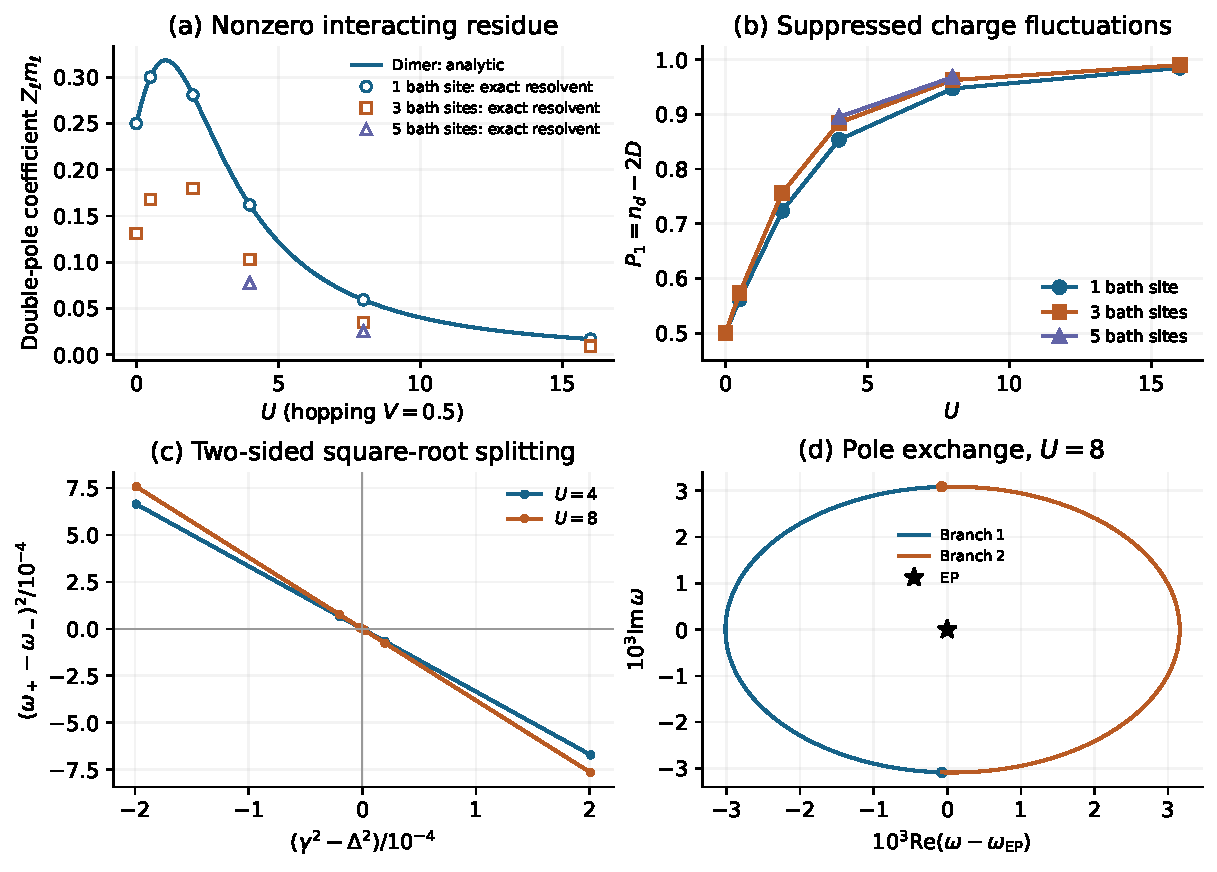
\includegraphics[width=\textwidth]{pt_control_checks.pdf}
\end{center}
\vspace{-6pt}
\small
\textbf{Checks.} Fourteen exact cases cover one and three bath sites at
$U=0,0.5,2,4,8,16$, and five bath sites at $U=4,8$.
For every selected doublet the nullities of $H-E$ and $(H-E)^2$ are
one and two. Direct contour integration gives the nonzero coefficient in
Eq.~(\ref{eq:residue}); halving the contour radius and doubling its mesh
preserves it. The third-order pole coefficient vanishes numerically.
Analytic dimer formulas, the $U=0$ one-body inverse, anticommutator sum rules,
direct versus Schur resolvents, and PT versus triangular-basis responses
provide independent checks. No many-body states are truncated.

At $U=4,8$ with three bath sites, two-sided splitting approaches
$4m_\ell^2(\Delta^2-\gamma^2)$. Two small loops in
$(\gamma,\eta)$, where $\eta\sigma_z$ is a real longitudinal field, give
squared-splitting winding $-1$ and pole exchange. The loops deliberately
leave the PT line. A real bath field $0.005\sigma_x$ preserves PT but splits
the poles at the old null-field condition: full spin covariance, not PT
alone, supplies the stronger restriction used here.

\textbf{What can now be stated.} The scalar-bath control has an interacting,
impurity-visible double pole with nonzero amplitude in a specified
single-occupancy finite-system setting. This is stronger than the previous
normalized-residue alignment audit.

\textbf{What remains separate.} The non-Hermitian core is imposed in this
control. No passive microscopic drive realization or complete Lindblad
steady state is derived here. Its discrete poles are not outgoing continuum
resonances. The original full-$k$ bath has spin structure outside the impurity
and does not obey the covariance assumption. Its interacting self-energy,
continuum convergence and outgoing continuation still need their own checks.
The singlet isolation gap and pole weight can vanish in limiting procedures.

\textbf{Prior work and novelty.} Interaction-stable symmetry-protected EPs
are already known: R.~Sch\"afer, J.~C.~Budich and D.~J.~Luitz,
\emph{Physical Review Research} \textbf{4}, 033181 (2022),
\href{https://doi.org/10.1103/PhysRevResearch.4.033181}{doi:10.1103/PhysRevResearch.4.033181}.
This note establishes the stated calculation, not priority for a new general
theorem. A literature comparison is needed before asserting novelty of this
particular impurity-residue result.

\textbf{Reproducibility.} The accompanying \texttt{REPORT.md}, Python scripts,
\texttt{table.csv}, and \texttt{results/} contain the derivation, raw checks,
contours, loops, and numerical residuals. The manuscript was not modified.
\end{document}
